\documentclass[french]{article}
\usepackage[utf8]{inputenc}
\usepackage[T1]{fontenc}
\usepackage{babel}
\usepackage{lmodern}
\usepackage{graphicx}
\usepackage{tikz}
\usepackage{fullpage}

\usepackage{float}

\usepackage{tabularx}

\usepackage{amsmath}
\usepackage{amsfonts}
\usepackage{amssymb}

\title{Algorithmique 2}
\date{}
\author{L3 RI}

\newcommand{\NP}{\mathrm{NP}}
\newcommand{\size}[1]{\vert #1 \vert}

\begin{document}
\maketitle
\tableofcontents

\section{NP-Complétude}

\subsection{Définitions}

\paragraph{Réduction} Soient $L_1$, $L_2$ des langages.
Une réduction polynomiale de $L_1$ à $L_2$ est une fonction $f$ calculable en temps polynomial telle que :
	\[ f(x) \in L_2 \Longleftrightarrow x \in L_1 \]
On note $L_1 \leq L_2$ ($L_1$ plus facile que $L_2$ = Si on sait résoudre $L_2$, on sait résoudre $L_1$)

\begin{figure}[H]
\center
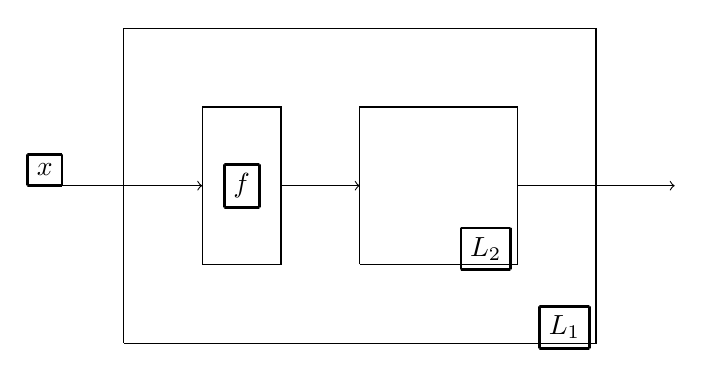
\begin{tikzpicture}
\draw (1,0) -- (1,4) -- (7,4) -- (7,0) -- (1,0);
\draw (2,1) -- (2,3) -- (3,3) -- (3,1) -- (2,1);
\draw (4,1) -- (4,3) -- (6,3) -- (6,1) -- (4,1);
\draw[->] (0,2) -- (2,2);
\draw[->] (3,2) -- (4,2);
\draw[->] (6,2) -- (8,2);
\node[draw,line width=-1] at (0,2.2) {$x$};
\node[draw,line width=-1] at (2.5,2) {$f$};
\node[draw,line width=-1] at (5.6,1.2) {$L_2$};
\node[draw,line width=-1] at (6.6,0.2) {$L_1$};
\end{tikzpicture}
\caption{Schéma de réduction de $L_1$ à $L_2$}
\end{figure}

\paragraph{Classe NP}Soit $L$ un langage. $L$ est dit dans la classe NP s'il existe une machine de Turing non-déterministe en temps polynomial par rapport à la taille de l'entrée qui décide $L$.

\paragraph{NP-Complétude} Soit $L$ un langage. $L$ est dit NP-dur si pour tout $L' \in \NP$, $L' \leq L$.
$L$ est dit NP-complet si $L \in \NP$ et $L$ est NP-dur.

\paragraph{Remarques} Si un problème NP-complet est dans P, alors P = NP. Pour montrer que $L'$ est NP-dur, il suffit de montrer qu'il existe $L$ NP-dur tel que $L \leq L'$.

\subsection{Satisfiabilité d'une formule}

\vspace{0.5cm}
\begin{tabularx}{\textwidth}{p{1cm}X}
\multicolumn{2}{c}{\textbf{Problème de décision : SAT}} \\ 
\emph{Entrée} & $\varphi$ formule de la logique propositionnelle \\ 
\emph{Sortie} & Oui si $\varphi$ est satisfiable, c'est-à-dire s'il existe une valuation $v$ des variables qui rend $\varphi$ vraie \\
\end{tabularx}

\paragraph{Théorème de Cook} SAT est NP-complet.

\vspace{0.5cm}
\begin{tabularx}{\textwidth}{X}
\multicolumn{1}{c}{\textbf{Problème de décision : $i$-SAT}} \\ 
Restriction de SAT à des formules en forme normale conjonctive (CNF) tel que chaque clause contient au plus $i$ littéraux \\
\end{tabularx}

\paragraph{Théorème} 3-SAT est NP-complet.

\paragraph{Théorème} 2-SAT est dans P.

\subsection{Ensembles indépendants dans un graphe}

\vspace{0.5cm}
\begin{tabularx}{\textwidth}{p{1cm}X}
\multicolumn{2}{c}{\textbf{Problème de décision : ENS\_INDEP}} \\ 
\emph{Entrée} & $G = (V, E)$ un graphe non-orienté et $k \in \mathbb{N}$ \\ 
\emph{Sortie} & Oui s'il existe $V' \subseteq V$ tel que $\size{V'} = k$ et $(V' \times V') \cap E = \varnothing$ \\
\end{tabularx}

\paragraph{Théorème} ENS\_INDEP est NP-complet

\section{Algorithmes d'approximation}

\section{Algorithmes probabilistes}

\section{Géométrie algorithmique}

\section{Algorithmes distribués}



\end{document}
